Jusqu'à présent nous nous sommes intéressés au système d'un point de vue globale. Nous passons désormais à une analyse détaillée de l'agent \cogito{}.

\subsection{Représentation des connaissances}
\label{subsection_representation_co}
	Les connaissances sont décrites en logique du première ordre. D'une part le plateau sera représenté comme un ensemble de faits et d'autres part les \og formes \fg{} seront exprimées par des règles dont l'hypothèse symbolise la sous structure à reconnaître et la conclusion un identifiant de cette forme.
	
	\subsubsection{Vocabulaire} 
	\begin{itemize}
	\item $isMine(x)$ : un qui m'appartient occupe la case $x$,
  	\item $isOpp(x)$ : un qui appartient à l'adversaire occupe la case $x$,
  	\item $isEmpty(x)$ : il n'y a pas de pion sur la case $x$,
  	\item $isEdge(x)$ : la case $x$ se trouve au bord du plateau,
  	\item $isCorner(x)$ : la case $x$ se trouve dans un coin du plateau,
  	\item $near(x,y)$ : les cases $x$ et $y$ sont adjacentes horizontalement, verticalement ou en diagonale,
  	\item $aligned(x,y,z)$ : les cases $x$, $y$ et $z$ sont sur la même ligne, colonne ou diagonale dans cet ordre (ou dans l'ordre inverse).
	\end{itemize}

\label{specs_voc_fol}

\subsection{Le package FOL}
\label{subsection_fol}

Le package \package{FOL}\footnote{FOL pour \og First Order Logic \fg{} (\og Logique du Premier Ordre \fg{} en Français). } contient l'ensemble des classes représentant des informations en logique du premier ordre.

\begin{itemize}
  \item \textbf{\class{\gls{Cbs}}} : \og Complete Board State \fg{}, c'est la version logique du premier ordre de \class{\gls{BoardMatrix}} définie section \vref{game_logic_shared},
  
  \item \textbf{\class{\gls{Rpbs}}} : \og Relevant Partial Board State \fg{}, classe qui décrit la configuration d'une sous-partie pertinente d'un plateau comme une règle logique. Elle correspond aux \og formes \fg{} extraites par le module de raisonnement qui doivent être reconnues dans les \class{\gls{CompleteBoardState}},
  
   \item \textbf{\class{\gls{Option_FOL}}} : c'est la version logique de la classe \class{Option},
   
   \item \textbf{\class{\gls{Choices_FOL}}} : elle est la version convertie par l'analyseur de \emph{Choices} (même structure, attributs décrits par des formules logiques) avec, en supplément, une liste de formes pertinentes, chacune associée à chaque plateau du paquet.
\end{itemize}


\subsection{Spécifications des classes \class{\gls{Cbs}} et \class{\gls{Rpbs}}}
\label{subsection_cbs_rpbs}

\begin{figure}[H] 
\centering
    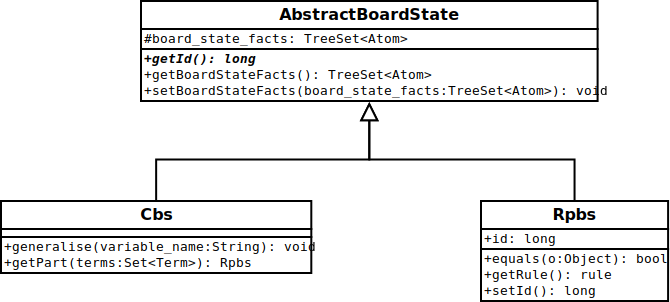
\includegraphics[width=\textwidth]{files/class_diagram/rpbs_cbs} 
\caption{Diagramme de classe des \class{\gls{Cbs}} et \class{\gls{Rpbs}}.} 
\label{img_diag_class_board_state}
\end{figure}

Les classes \class{\gls{Cbs}} et \class{\gls{Rpbs}} représentent respectivement un plateau et une sous configuration d'un plateau dans le format logique décrit dans la section \vref{subsection_representation_co}. 